% !TeX encoding = UTF-8
\documentclass[a4paper,12pt]{article}
\usepackage{ctex,geometry,graphicx,tikz,setspace,paralist,fancyhdr,caption,ulem,amsmath,verbatim}
\geometry{
	left=2cm,
	right=2cm,
	top=2cm,
	bottom=2cm,}
\renewcommand{\maketitle}{
	\begin{titlepage}
		\begin{center}
			
\includegraphics[width=0.4\textwidth]{1_1.png} % 插入你的公司/机构logo
			\vspace{4cm}
			
			\zihao{1} \textbf{数值计算\\期中大作业} \\
			\vspace{2cm}
			
			\zihao{3} 专业:\uline{通信工程} \\
			\vspace{0.5cm} 
			\zihao{3} 学号:\uline{22309080} \\
			\vspace{0.5cm} 
			\zihao{3} 姓名:\uline{梁倍铭} \\
			\vspace{0.5cm} 
			\zihao{3} 时间:\uline{2023.12.21} \\
			\vfill
		\end{center}
	\end{titlepage}
}
\begin{document}
	\maketitle
	\tableofcontents
	\newpage
	\large
	\onehalfspacing
	\section{MIMO系统简介}
	MIMO全称是multiple-in multiple-out,多输入多输出。示意图如图1,具有$N_T$根发射天线和$N_R$根接收天线,且$N_R>N_T$,数据在$N_T$个等长的数据子流(称为层)中进行解复用。这些子流被映射成M-PSK或M-QAM符号,或者,可以使用前向纠错(FEC)码在映射之前对数据子流进行编码。\par 
	\begin{figure}[h]
		\centering
		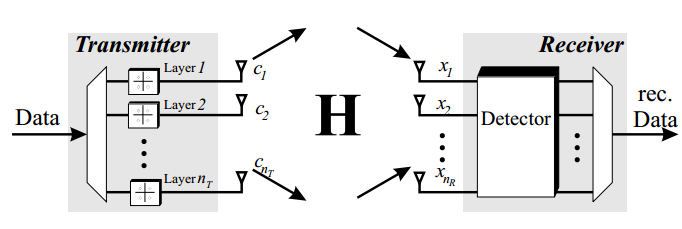
\includegraphics[width=0.5\textwidth]{1.png}
		\caption{MIMO系统示意图}
	\end{figure}
	用$c=\begin{pmatrix}
		c_1&c_2&\dots &c_{nt}
	\end{pmatrix}^\top $来表示发射的信号,用$x=\begin{pmatrix}
		x_1&x_2& \dots &x_{nr}
	\end{pmatrix}$来表示接收到的信号。信道H的大小为$N_T*N_R$,信道H可表示为$$H=\begin{pmatrix}
		h_{1,1}& \dots & h_{1,nT} \\
		\cdots &	\cdots	& \cdots \\
		h_{nR,1}& \dots & h_{nR,nT}
	\end{pmatrix}$$
	由于两篇论文所使用的符号不尽相同,这里采用第一篇论文的符号进行统一描述,用v来表示接收天线中的高斯白噪声,
	$v=\begin{pmatrix}
		v_1&v_2& \dots & v_{NR}
	\end{pmatrix}^\top$,因此,整个系统可以用$x=Hc+v$来描述。\par 
	其中我们假设假设所有天线每维的方差 N0=2 的不相关高斯白噪声。传输的符号被归一化,使得每比特的平均接收能量为一。我们假设静态平坦衰落环境,即信道矩阵 H 在帧内保持不变,并且在帧与帧之间独立变化。假定不同的衰落增益是不相关的并且接收机完全了解这些增益。
	\section{《Efficient Algorithm for Detecting Layered Space-Time Codes》中算法的复现}
	\subsection{简介}
	分层空时码的设计是为了在瑞利衰落环境中利用多天线系统的容量优势。在《Efficient Algorithm for Detecting Layered
	Space-Time Codes》一文中,提出了一种基于排序QR分解的新高效检测算法。与需要多次计算信道矩阵伪逆的标准检测算法相比,它只需要一小部分计算量。导出的算法不限于分层时空架构,而是通常可用于矢量信道系统中的检测。\par 
	本部分将用matlab软件对V-BLAST、QR 分解及QR 分解的排序算法进行仿真复现,并对其进行性能分析。
	\subsection{各算法的分析及仿真代码}
	\subsubsection{V-BLAST算法分析及仿真}
	从上文的描述可以看出,接收信号是nT个发射信号的线性组合。在接收器处恢复$N_T$信号的最佳方法是最大似然检测,但由于其巨大的复杂性,这是不可行的。\par 
	Foschini等人提出了一种连续干扰消除技术,该技术通过使用迫零(ZF)归零向量对接收信号向量进行线性加权来消除干扰源。在每个检测步骤中,除了一个信号之外的所有信号都被视为干扰源。通过将调零矢量应用于干扰消除,这些信号的影响被消除,目标信号被检测到并随后从接收到的信号矢量中减去(干扰消除)。算法伪代码如图2,matlab代码如图3
	\begin{figure}[h]
		\centering
		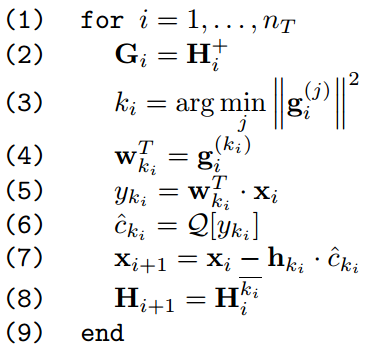
\includegraphics[width=0.5\textwidth]{2.png}
		\caption{V-blast伪代码}
	\end{figure}
	\begin{figure}[h]
		\centering
		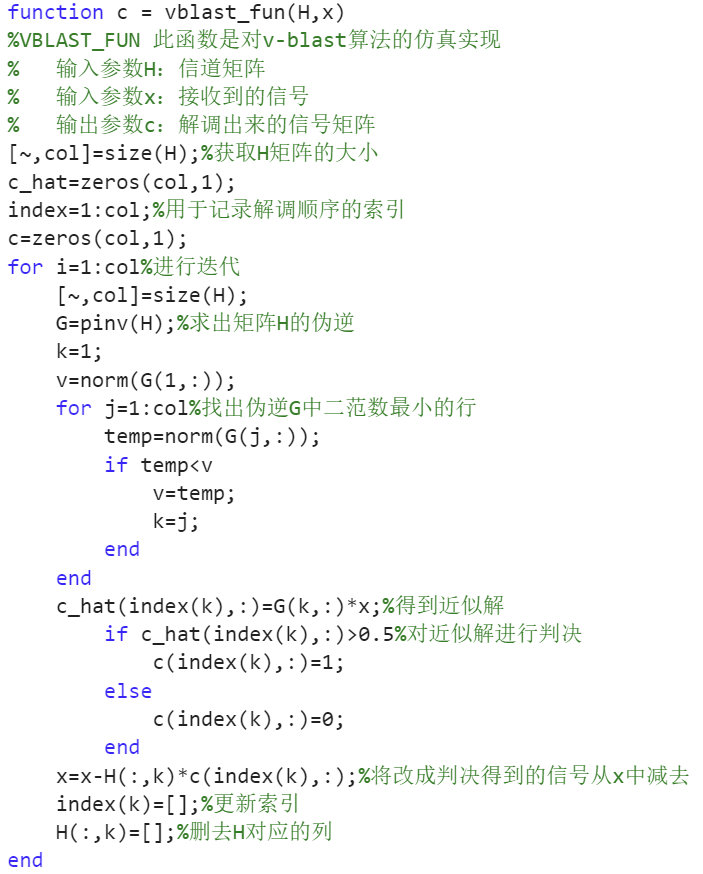
\includegraphics[width=0.8\textwidth]{3.png}
		\caption{V-blast matlab代码}
	\end{figure}
	\newpage
	\subsubsection{Unsorted QRD算法分析及仿真}
	由于V-BLAST算法的复杂度较高,我们可以通过变换信道矩阵H避免矩阵的求逆,获得较低的计算复杂度。根据论文,该算法首先对信道矩阵H进行了QR分解,即$$H=Q\cdot R$$
	其中Q为酉矩阵,R为上三角阵。将接收到的信号左乘$Q^H$得到$n_T\times 1$修正的接收信号向量
	$$y=Q^H\cdot x=R\cdot c+\eta$$
	由于Q是正交归一化的,所以$\eta$的统计特性保持不变,y的第k个元素为
	$$y_k=r_{k,k}\cdot c_k+\eta +d_k$$
	其中$d_k$为干扰项
	$$d_k=\sum_{i=k+1}^{n_T}r_{k,i}\cdot c_i $$
	从第$n_T$层开始检测,即可逐层获取发射信号。伪代码如图4,matlab代码如图5。
	\begin{figure}[h]
		\centering
		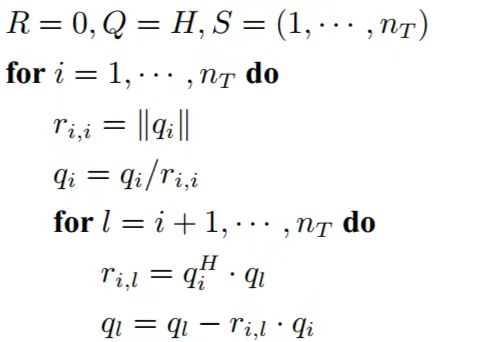
\includegraphics[width=0.6\textwidth]{1.jpg}
		\caption{Unsorted QRD伪代码}
	\end{figure}
	\begin{figure}[h]
		\centering
		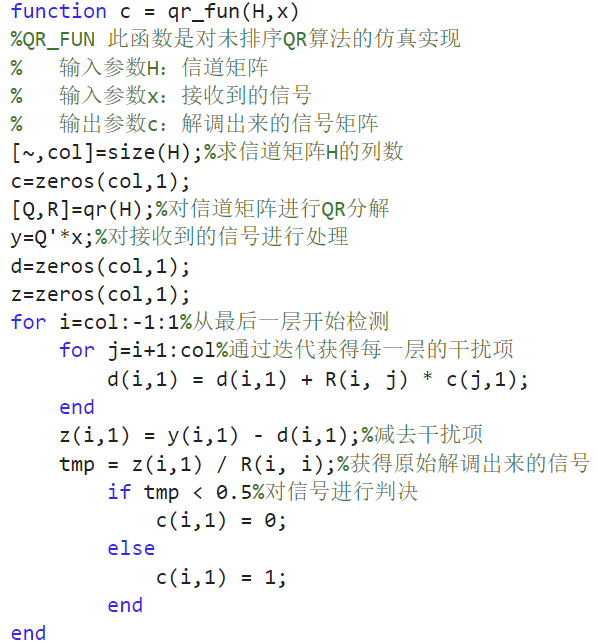
\includegraphics[width=0.8\textwidth]{4.png}
		\caption{Unsorted QRD matlab代码}
	\end{figure}
	\newpage
	\subsubsection{Sorted QRD算法分析及仿真}
	由于QR算法不能决定最先检验层,而最先检验层会影响后续检验的精确性。而Sorted QR则是非常有效的新方法,其错误性能接近 V-BLAST。它基本上是改进的 Gram-Schmidt 算法的扩展,即在每个正交化步骤中对 H 的列进行排序。\par 
	根据论文,上三角阵R的对角元素$|r_{k,k}|$与信号的估计误差成反比,所以在每次检测中先选取最大的$r_{k,k}|$来检测信号,来做到误差最小化。伪代码如图6,matlab代码如图7。
	\begin{figure}
		\centering
		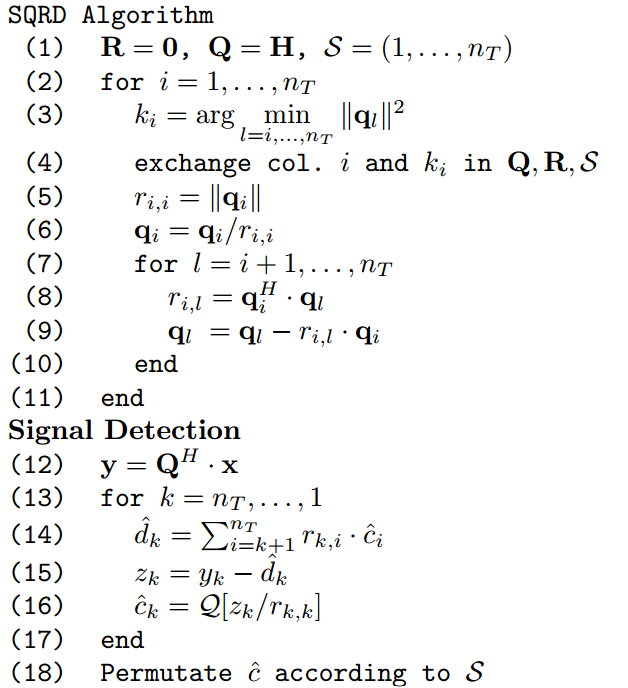
\includegraphics[width=0.4\textwidth]{5.png}
		\caption{Sorted QRD伪代码}
	\end{figure}
	\begin{figure}
		\centering
		\begin{minipage}{0.4\textwidth}
			\centering
			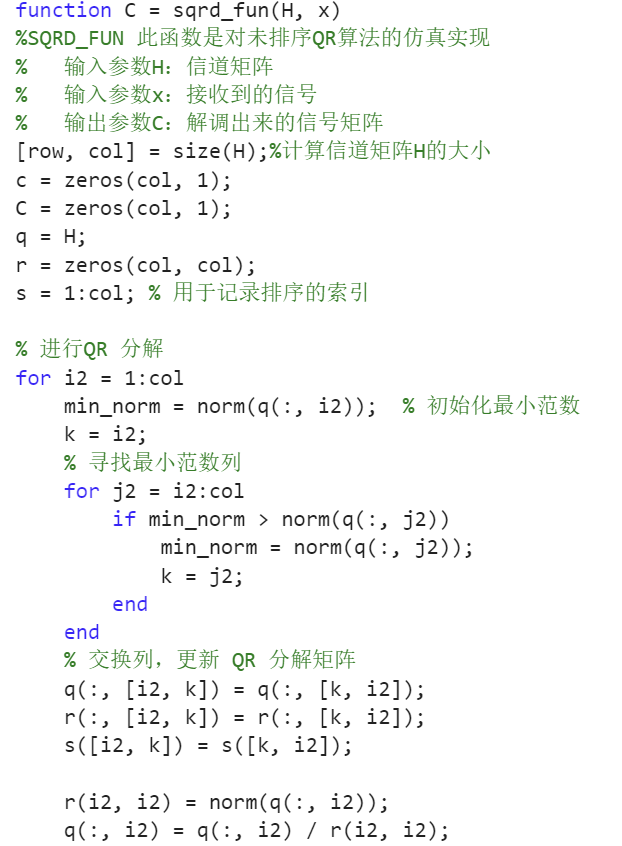
\includegraphics[width=\textwidth]{6.png}
		\end{minipage}
		\qquad
		\begin{minipage}{0.4\textwidth}
			\centering
			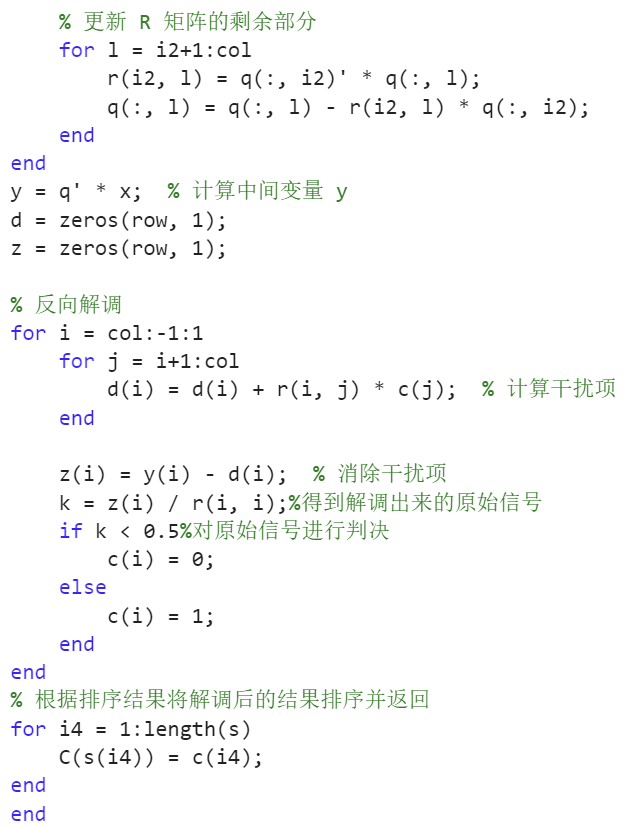
\includegraphics[width=\textwidth]{7.png}
		\end{minipage}
		\caption{Sorted QRD matlab代码}
	\end{figure}
	\newpage
	\subsection{仿真测试}
	\subsubsection{误码率测试}
	\paragraph{测试思路}
	通过假设在满足$N_T>N_R$条件的天线数,通过设定不同的信噪比,计算不同算法的误码率,来对各个算法进行分析,进行误码率计算的matlab代码如图8。由于计算量巨大,使用了matlab的并行计算工具包Parallel Computing Toolbox减少代码的运行时间。\par 
	\begin{figure}[h]
		\centering
		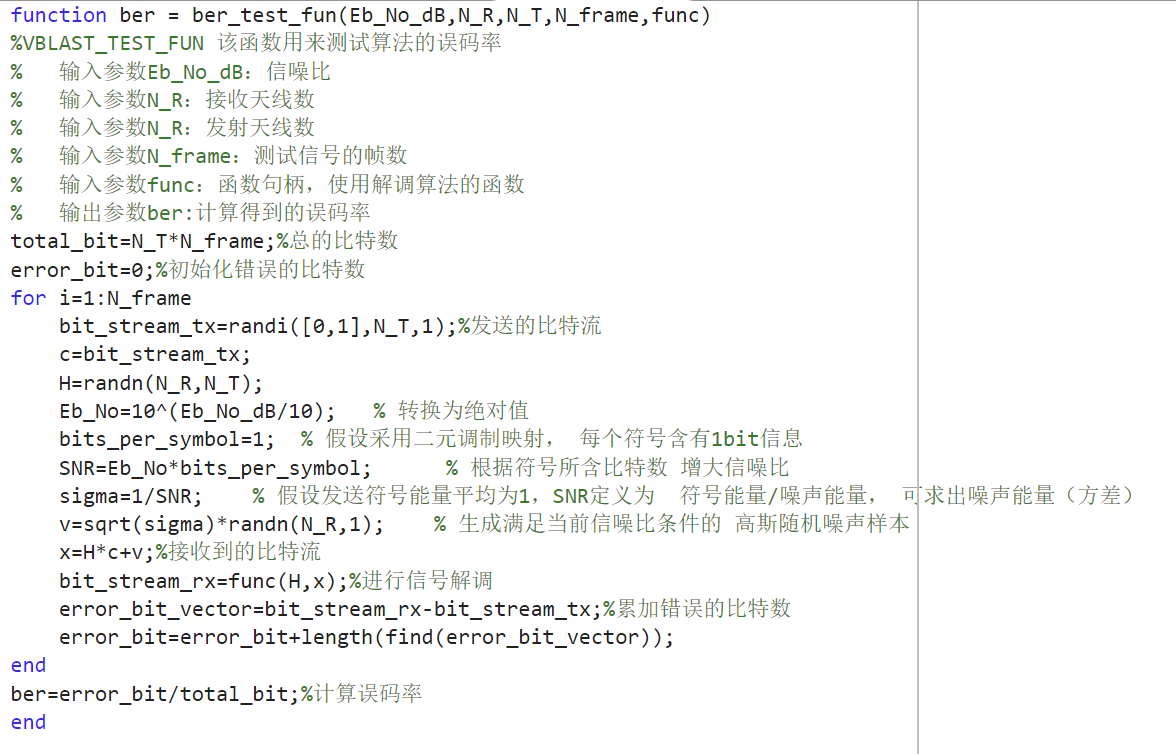
\includegraphics[width=0.8\textwidth]{8.png}
		\caption{误码率测试代码}
	\end{figure}
	\paragraph{测试结果}
	对不同情况的误码率仿真测试结果如下:
	\begin{enumerate}
		\item $n_T=8,n_R=12$,信噪比为0-20dB,测试帧数为1000000,结果如图9
		\item $n_T=4,n_R=6$,信噪比为0-20dB,测试帧数为1000000,结果如图10
		\begin{figure}[h]
			\centering
			\begin{minipage}{0.4\textwidth}
				\centering
				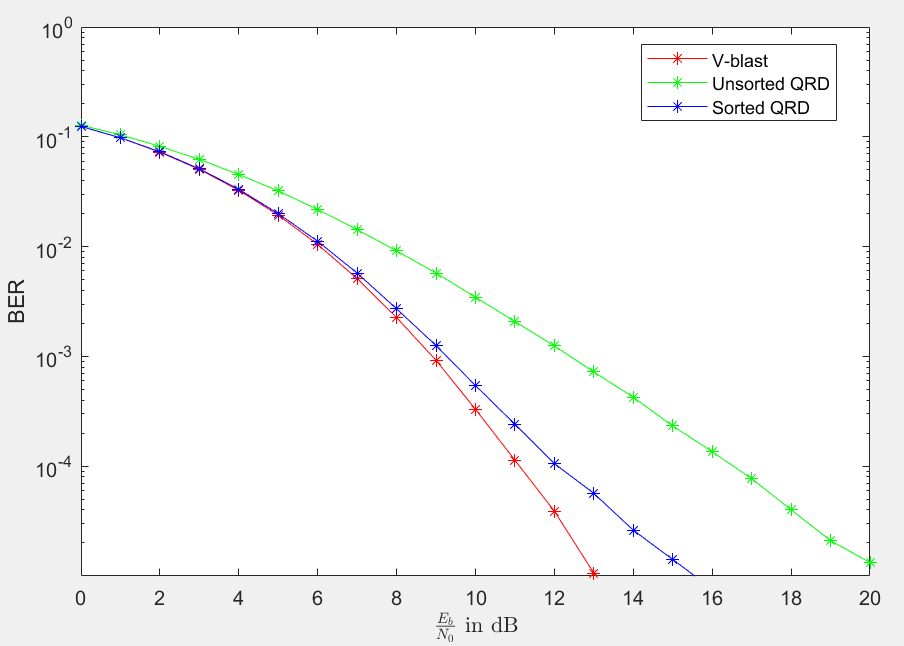
\includegraphics[width=\textwidth]{9.png}
				\caption{$n_T=8,n_R=12$,信噪比为0-20dB,测试帧数为1000000的误码率测试结果图}
			\end{minipage}
			\qquad
			\begin{minipage}{0.4\textwidth}
				\centering
				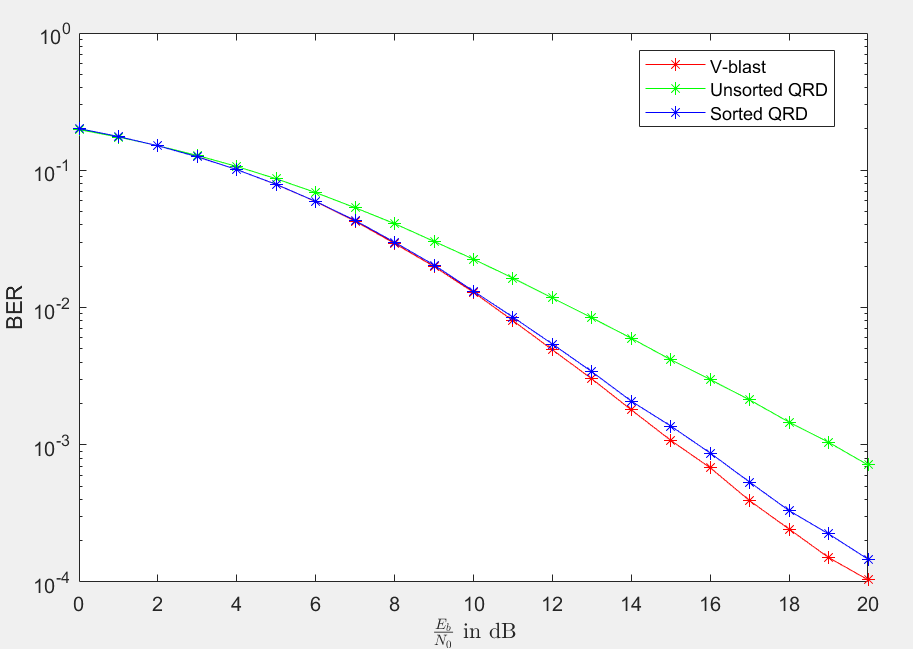
\includegraphics[width=\textwidth]{10.png}
				\caption{$n_T=4,n_R=6$,信噪比为0-20dB,测试帧数为1000000的误码率测试结果图}
			\end{minipage}
		\end{figure}
	\end{enumerate}
	\newpage
	\subsubsection{误帧率测试}
	\paragraph{测试思路}
	通过假设在满足$N_T>N_R$条件的天线数,通过设定不同的信噪比,假定一定的帧数,采用类似误码率的统计方法,来对各个算法进行分析,进行误码率计算的matlab代码如图11。由于计算量巨大,使用了matlab的并行计算工具包Parallel Computing Toolbox减少代码运行时间。\par
	\begin{figure}[h]
		\centering
		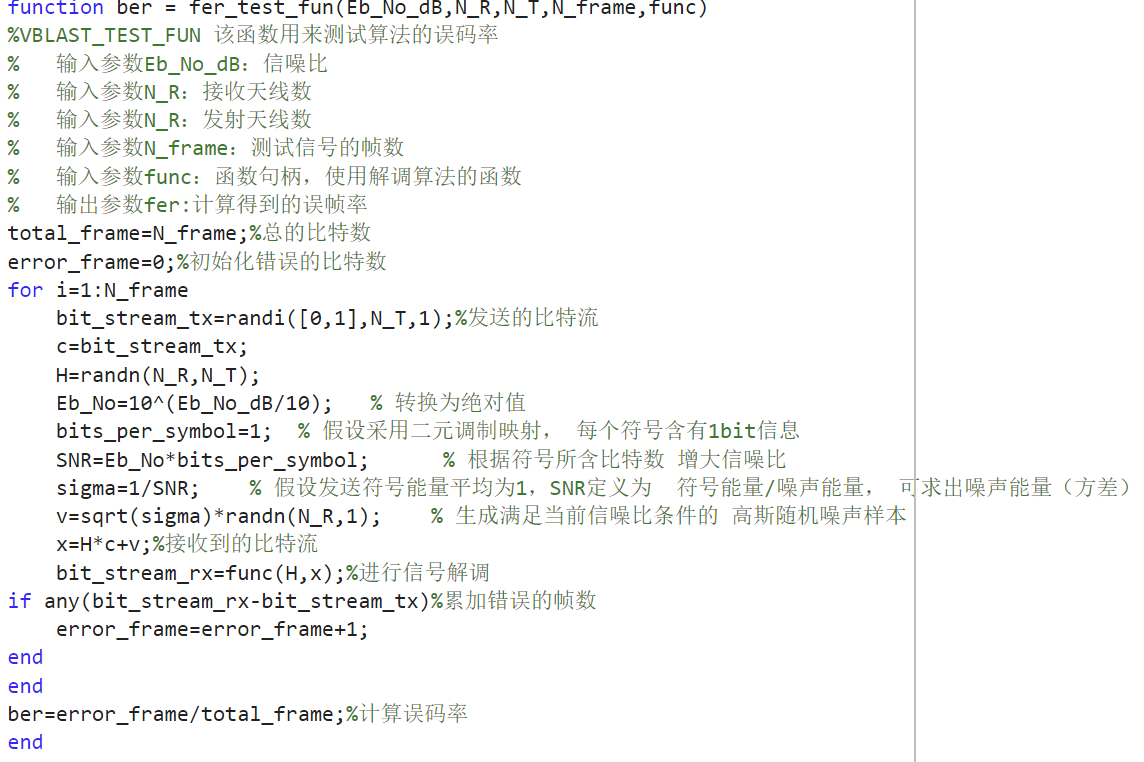
\includegraphics[width=0.8\textwidth]{11.png}
		\caption{误帧率测试代码}
	\end{figure}
	\paragraph{测试结果}
	对不同情况的误帧率仿真测试结果如下:
	\begin{enumerate}
		\item $n_T=8,n_R=12$,信噪比为0-20dB,测试帧数为1000000,如图12
		\item $n_T=4,n_R=6$,信噪比为0-20dB,测试帧数为1000000,如图13
		\begin{figure}[h]
			\centering
			\begin{minipage}{0.4\textwidth}
				\centering
				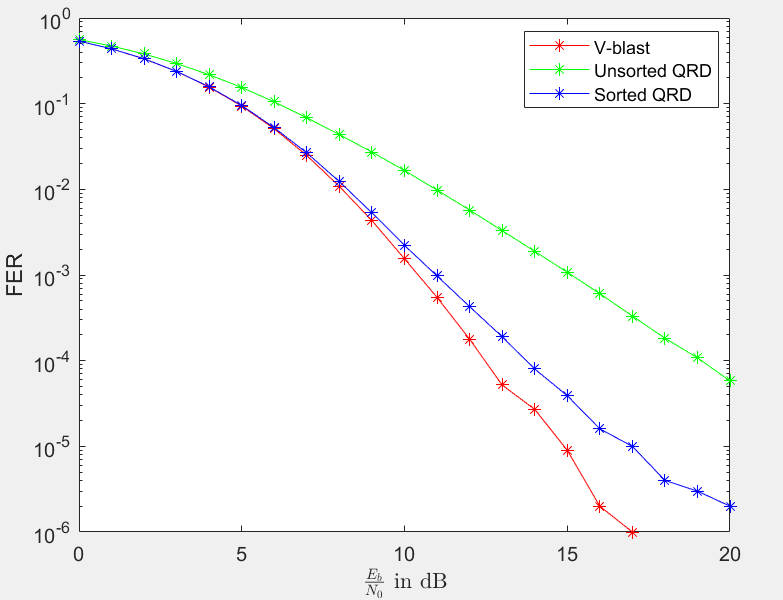
\includegraphics[width=\textwidth]{12.png}
				\caption{$n_T=8,n_R=12$,信噪比为0-20dB,测试帧数为1000000的误帧率测试结果图}
			\end{minipage}
			\qquad
			\begin{minipage}{0.4\textwidth}
				\centering
				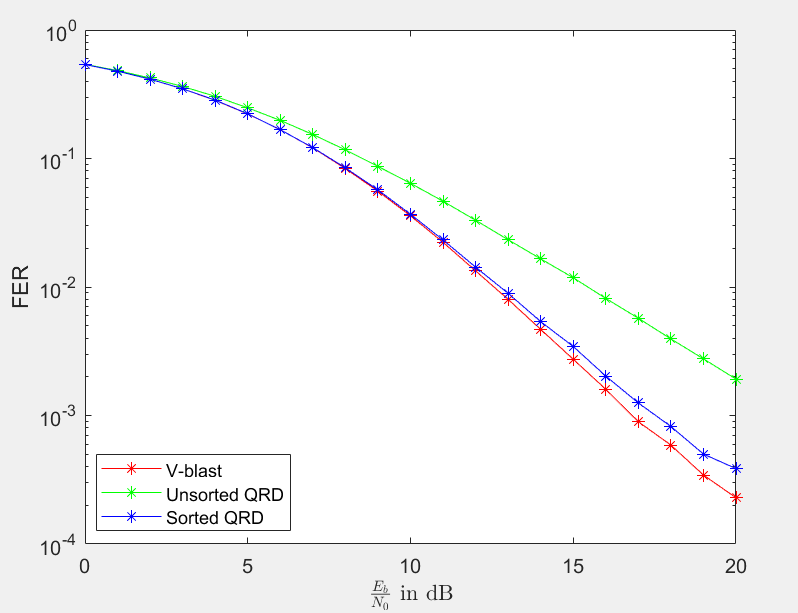
\includegraphics[width=\textwidth]{13.png}
				\caption{$n_T=4,n_R=6$,信噪比为0-20dB,测试帧数为1000000的误帧率测试结果图}
			\end{minipage}
		\end{figure}
	\end{enumerate}
	\newpage
	\subsubsection{结果分析}
	从仿真结果可以看出,在相同的信噪比下,发射天线和接收天线的数目增加时可以降低误码率,因此我们可以在MIMO系统中增加发射天线和接收天线的数量,来有效降低误码率。但是在实际应用中,收发天线的数目往往是受到限制的,特别是在移动终端中,而且随着天线数目的增加,计算量随之增多,会加大系统的功耗,因此有必要探寻高效的算法来降低误码率。\par 
	根据仿真结果图,三种算法中V-BLAST算法的误码率和误帧率在不同的信噪比下一直保持在较小水平,QR分解算法的误码率误帧率显著高于其他两种算法,说明QR分解的检测性能略差,但对QR分解进行排序后,误码率和误帧率有了一定降低,性能得到显著提升,结合算法的复杂度,V-BLAST算法的复杂度最高,换来的是精确的结果,而QR算法精度的损失,获得了最快的运行速度,而SQRD在保持较高的精度情况下,运算复杂度只比QR算法有微弱的增加,综上,SQRD算法的综合性能最好。
	\newpage
	\section{《MMSE Extension of V-BLAST based on Sorted QR Decomposition》中算法的复现}
	\subsection{简介}
	V-BLAST架构利用了多个天线系统的容量优势,使用垂直分层编码结构,其中独立的代码块(称为层)与特定的发射天线相关联。在接收器处,这些层通过连续干扰消除技术进行检测,该技术通过使用迫零归零向量 (ZF-BLAST) 对接收信号向量进行线性加权来消除干扰源。这种连续检测需要多次计算伪逆,这是一项计算成本高昂的任务。\par 
	在《MMSE Extension of V-BLAST based on
	Sorted QR Decomposition》一文中,作者提出了基于QR分解的MMSE算法,能够有效降低算法复杂度并明显提高算法复杂度,本部分将用matlab软件实现对ZF、MMSE、MMSE-QRD和MMSE-SQRD的仿真,并进行性能分析。
	\subsection{各算法分析及仿真代码}
	\subsubsection{Zero-Forcing Detector (ZF)算法分析及仿真}
	对于线性信号,ZF算法是指先对对信道矩阵求伪逆得到G,如何将接收到的信号x与G相乘,即
	$$G=H^{+}=(H^HH)^{-1}H^H$$
	$$\hat{c}=Gx$$
	然后对所有层进行并行决策。当$H^HH$的特征值较小时,会因噪声放大而导致较大的误差,这种效应在具有相同数量的发射和接收天线的系统中尤其明显。matlab代码如图14。
	\begin{figure}[h]
		\centering
		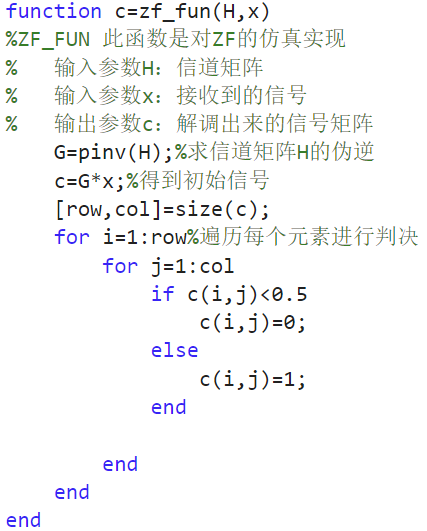
\includegraphics[width=0.6\textwidth]{14.png}
		\caption{ZF matlab代码}
	\end{figure}
	\newpage
	\subsubsection{MMSE算法分析及实现}
	如文中所述,ZF算法没有考虑到噪声的影响,当$H^HH$的特征值较小时,会因噪声放大而导致较大的误差,为了提高检测性能,MMSE算法能够最小化实际传输符号与线性检测器输出之间的均方误差 (MSE),并得出滤波器矩阵:
	$$G_{MMSE}=(H^HH+\sigma^2I_{nT})^{-1}H^H$$
	进而得到检测信号:
	$$\hat{c}_{MMSE}=H^{+}x$$
	matlab代码如图15。
	\begin{figure}[h]
		\centering
		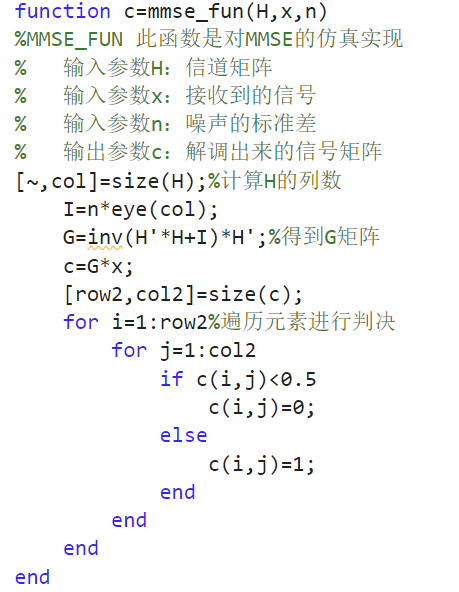
\includegraphics[width=0.6\textwidth]{15.png}
		\caption{MMSE matlab代码}
	\end{figure}
	\newpage
	\subsubsection{MMSE-QR算法分析及实现}
	将MMSE算法和QR算法进行结合,考虑噪声的影响,同时对信道矩阵进行QR分解,避免求伪逆。
	算法过程如下:\par
	假设噪声方差为$\sigma$,可以将信道矩阵H扩展为$\underline{H}=\begin{pmatrix}
		H\\ \sigma_{n}I_{nT},
	\end{pmatrix}$,而后对其QR分解,采用上面提到的QR分解算法进行计算即可。matlab代码如图16。
	\begin{figure}[h]
		\centering
		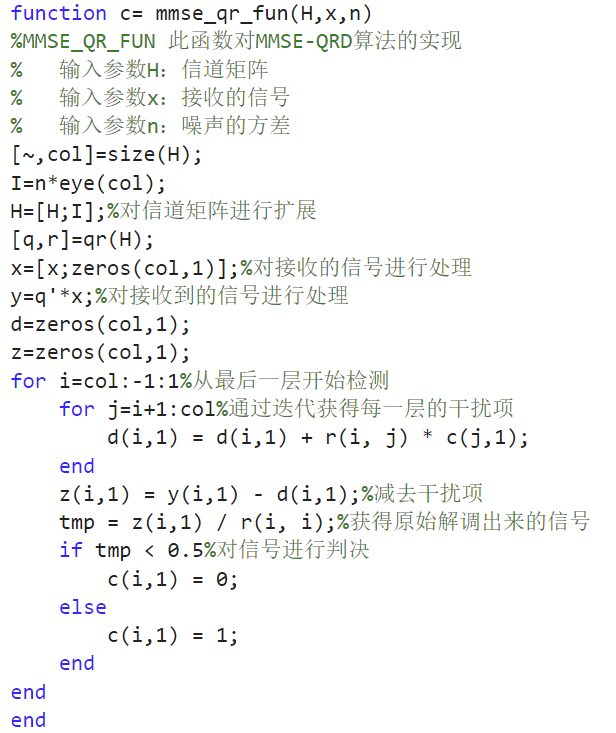
\includegraphics[width=0.6\textwidth]{16.png}
		\caption{MMSE-QRD matlab代码}
	\end{figure}
	\newpage
	\subsubsection{MMSE-SQRD算法的分析及实现}
	同样地,由于QR分解的误码率较高,因此可以考虑每次能够选取最大的$|k_{r,r}|$进行检测,这样可以获得更低的误码率。同时,我们与上述算法一样,将H矩阵扩展,并用SQRD来计算,可以获得较为精确的发射信号c。matlab代码如图17。
	\begin{figure}[h]
		\centering
		\begin{minipage}{0.4\textwidth}
			\centering
			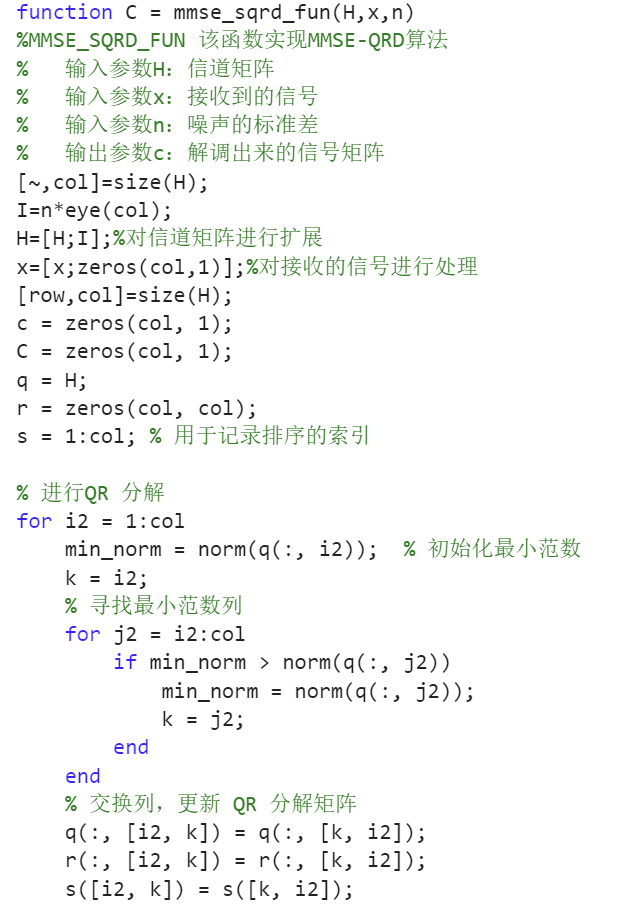
\includegraphics[width=\textwidth]{17.png}
		\end{minipage}
		\qquad
		\begin{minipage}{0.4\textwidth}
			\centering
			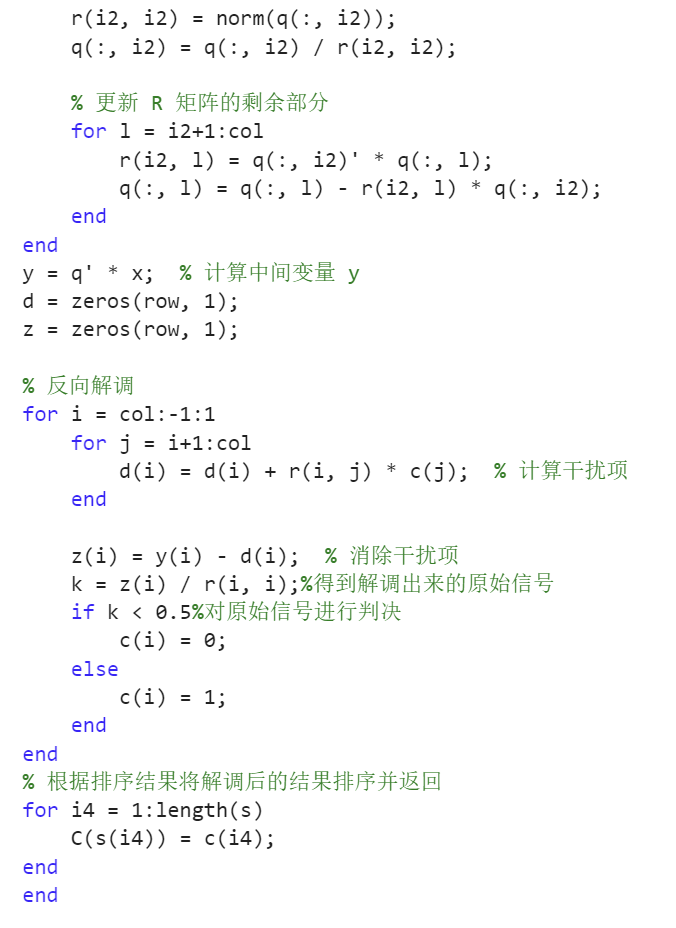
\includegraphics[width=\textwidth]{18.png}
		\end{minipage}
		\caption{MMSE-SQRD matlab代码}
	\end{figure}
		\newpage
	\subsection{仿真测试}
	采用与上一部分相同的方式,分别进行四种算法的误码率和误帧率测试。然后比较这几种算法在相同信噪比下的误码率来进行性能分析。
	\subsubsection{误码率测试}
	\paragraph{测试思路}
	通过假设在满足$N_T>N_R$条件的天线数,通过设定不同的信噪比,在该信噪比下,用错误的比特数除以总比特数,得到不同算法的误码率,来对各个算法进行分析。matlab代码如图18。由于计算量巨大,使用了matlab的并行计算工具包Parallel Computing。 Toolbox\par 
	\begin{figure}[h]
		\centering
		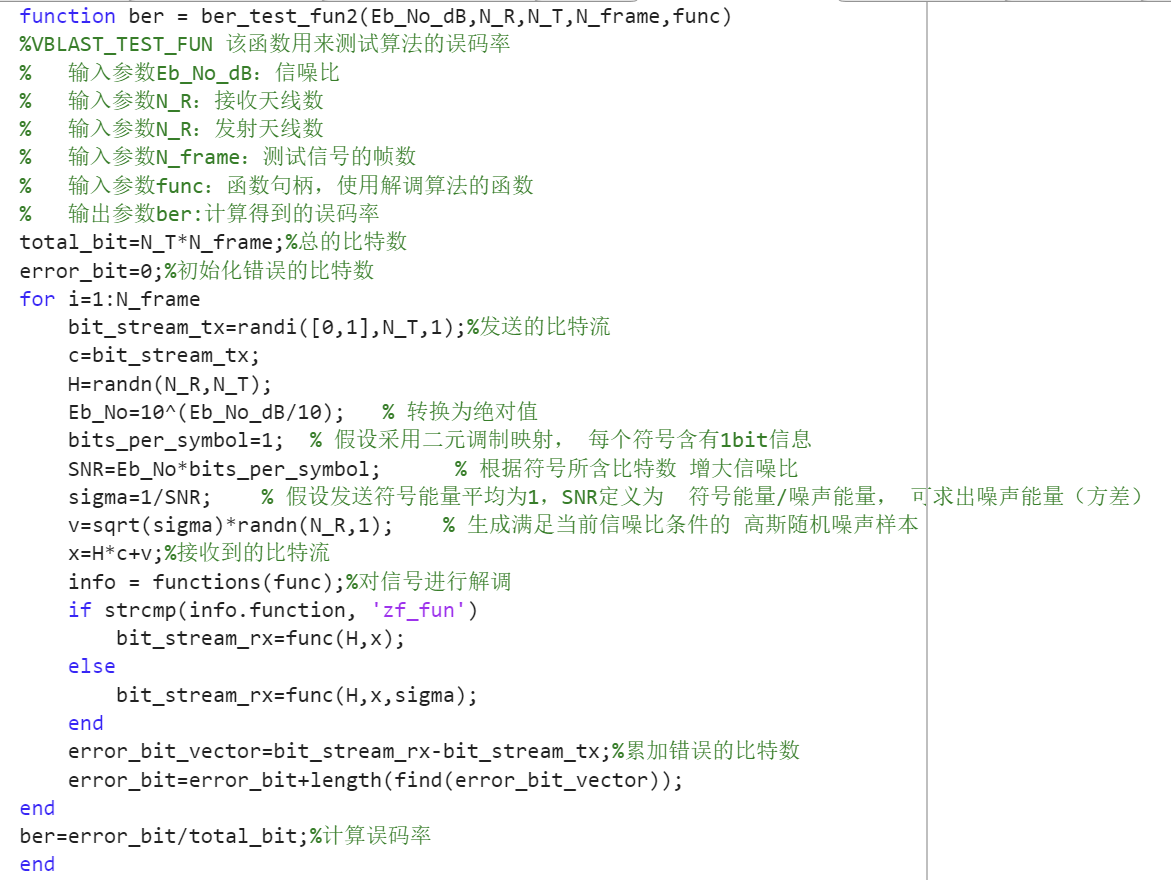
\includegraphics[width=0.8\textwidth]{19.png}
		\caption{误码率测试代码}
	\end{figure}
	\newpage
	\paragraph{测试结果}
	对不同情况的误码率仿真测试结果如下:
	\begin{enumerate}
		\item $n_T=8,n_R=12$,信噪比为0-20dB,测试帧数为1000000,结果如图19
		\item $n_T=4,n_R=6$,信噪比为0-20dB,测试帧数为1000000,结果如图20
		\begin{figure}[h]
			\centering
			\begin{minipage}{0.4\textwidth}
				\centering
				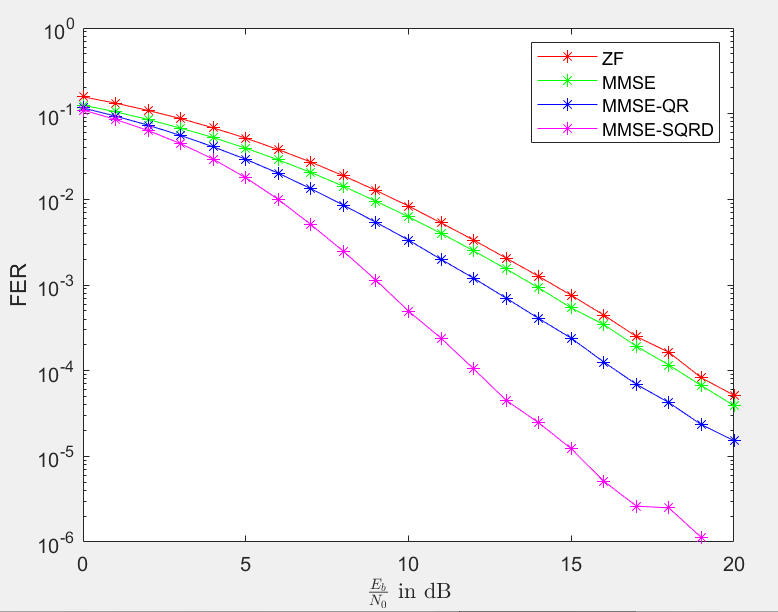
\includegraphics[width=\textwidth]{20.png}
				\caption{$n_T=8,n_R=12$,信噪比为0-20dB,测试帧数为1000000的误码率测试结果图}
			\end{minipage}
			\qquad
			\begin{minipage}{0.4\textwidth}
				\centering
				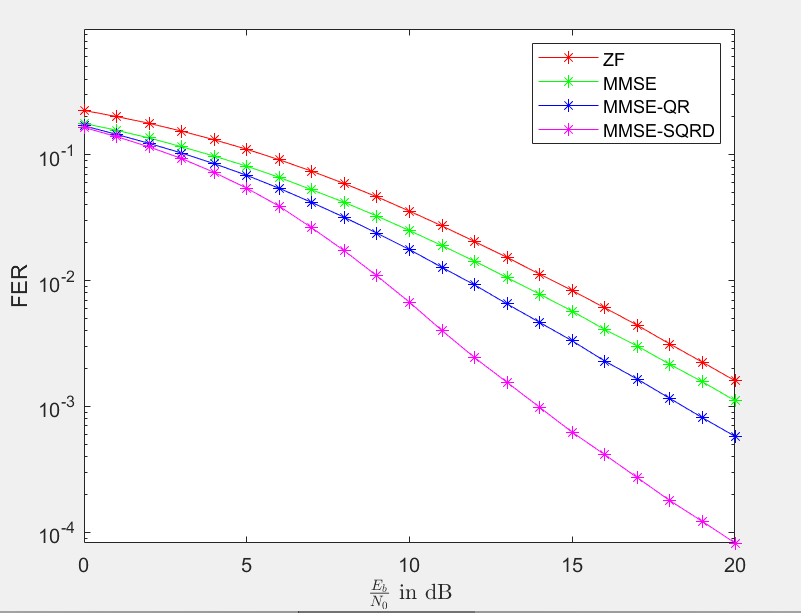
\includegraphics[width=\textwidth]{21.png}
				\caption{$n_T=4,n_R=6$,信噪比为0-20dB,测试帧数为1000000的误码率测试结果图}
			\end{minipage}
		\end{figure}
	\end{enumerate}
	\newpage
	\subsubsection{误帧率测试}
	\paragraph{测试思路}
	通过假设在满足$N_T>N_R$条件的天线数,通过设定不同的信噪比,假定一定的帧数,采用类似误码率的统计方法,计算得到误帧率。然后通过比较误帧率和计算复杂度来对各个算法进行分析,进行误帧率计算的matlab代码如图21。由于计算量巨大,使用了matlab的并行计算工具包Parallel Computing Toolbox。\par
	\begin{figure}[h]
		\centering
		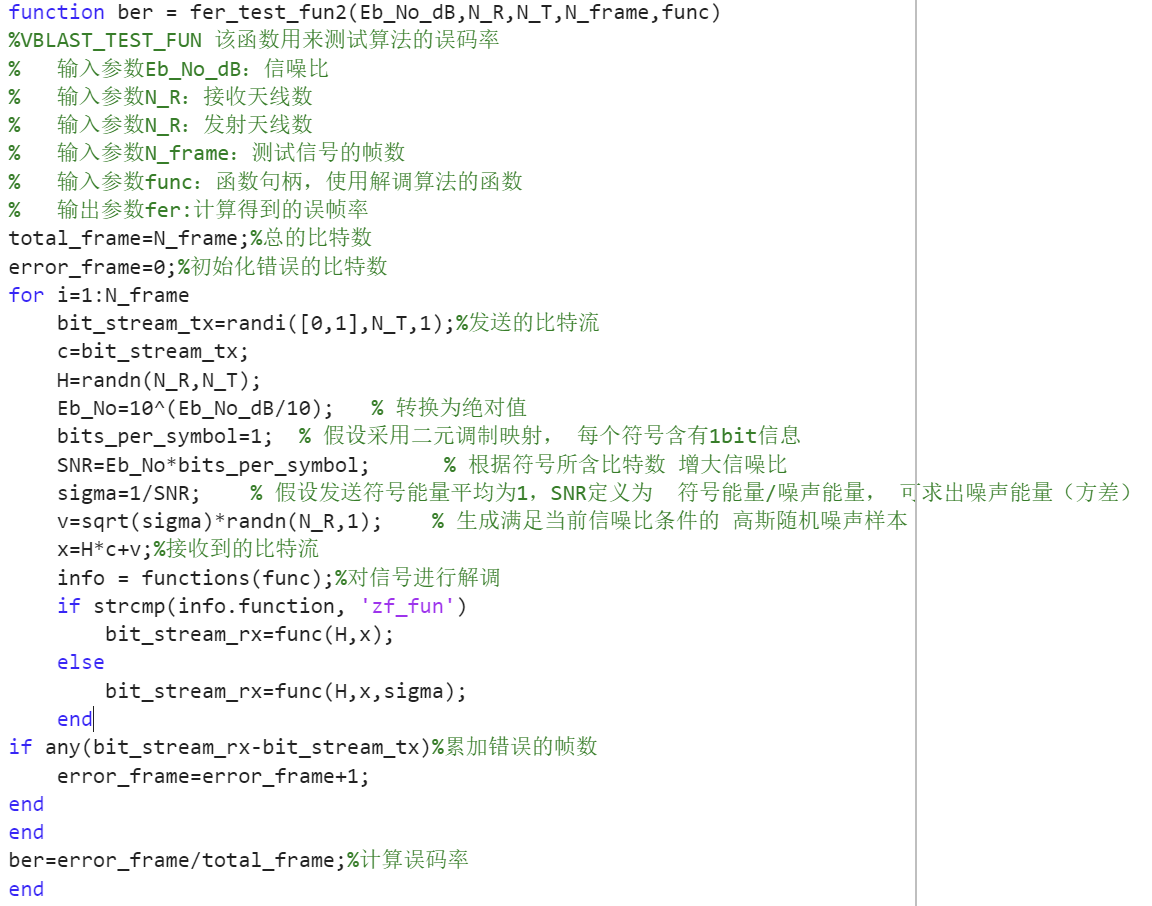
\includegraphics[width=0.9\textwidth]{22.png}
		\caption{误帧率测试代码}
	\end{figure}
	\paragraph{测试结果}
	对不同情况的误帧率仿真测试结果如下:
	\begin{enumerate}
		\item $n_T=8,n_R=12$,信噪比为0-20dB,测试帧数为1000000,如图22
		\item $n_T=4,n_R=6$,信噪比为0-20dB,测试帧数为1000000,如图23
		\begin{figure}[h]
			\centering
			\begin{minipage}{0.4\textwidth}
				\centering
				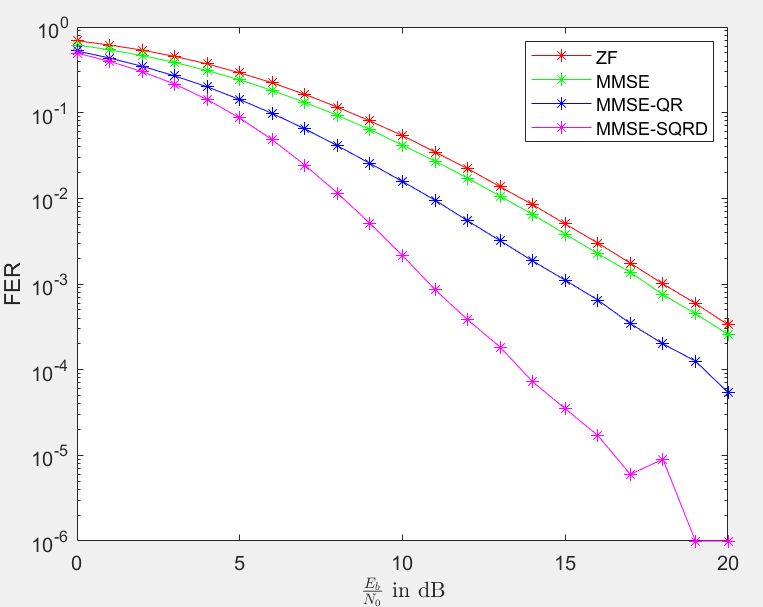
\includegraphics[width=\textwidth]{23.png}
				\caption{$n_T=8,n_R=12$,信噪比为0-20dB,测试帧数为1000000的误帧率测试结果图}
			\end{minipage}
			\qquad
			\begin{minipage}{0.4\textwidth}
				\centering
				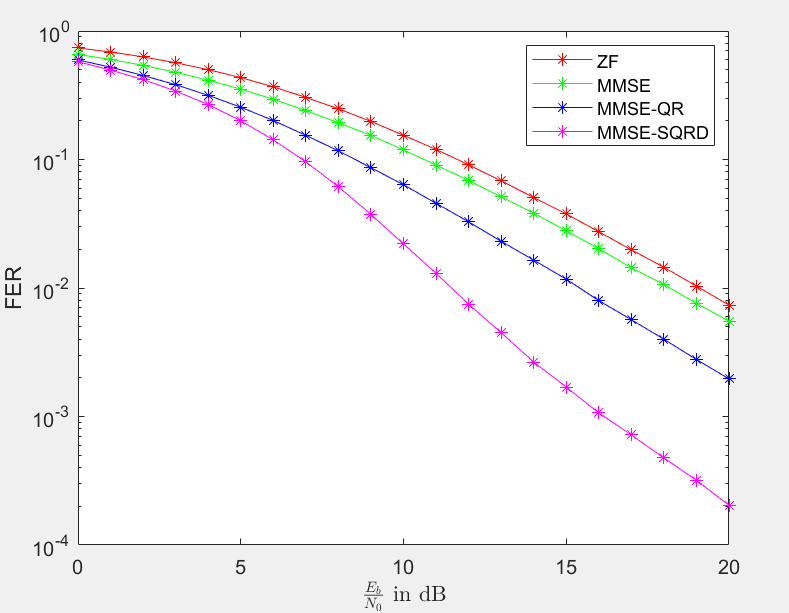
\includegraphics[width=\textwidth]{24.png}
				\caption{$n_T=4,n_R=6$,信噪比为0-20dB,测试帧数为1000000的误帧率测试结果图}
			\end{minipage}
		\end{figure}
	\end{enumerate}
	\newpage
	\subsubsection{结果分析}
	从得到的图像可以看出,ZF算法是这四个算法中误码率最高的,因为其没有考虑到噪声的影响,而MMSE算法考虑到了噪声的影响,所以误码率有所下降,但是其需要对H求逆运算,所以复杂度较高。通过考虑对H进行QR分解,可以降低复杂度,对QR分解进行排序,可以进一步降低误码率。因此,采用MMSE-SQRD算法可以获得较高的性能。
	\section{最大似然算法的实现}
	\subsection{简介}
	通过阅读资料,该算法的基本思想是通过比较接收到的信号与各种可能发送信号序列之间的似然性,来确定最可能的发送序列。它假设了接收端知道发送信号的统计特性以及噪声的统计特性,并基于这些假设进行数据检测。最似然检测算法能够以很高的准确度来检测出发射信号,因为最似然检测算法计算出信号所有可能的集合,并通过最小距离判决来寻找出最接近的信号,高精度的代价是计算的复杂度更高。
	\subsection{算法的实现}
	用matlab实现的代码如图24
	\begin{figure}[h]
		\centering
		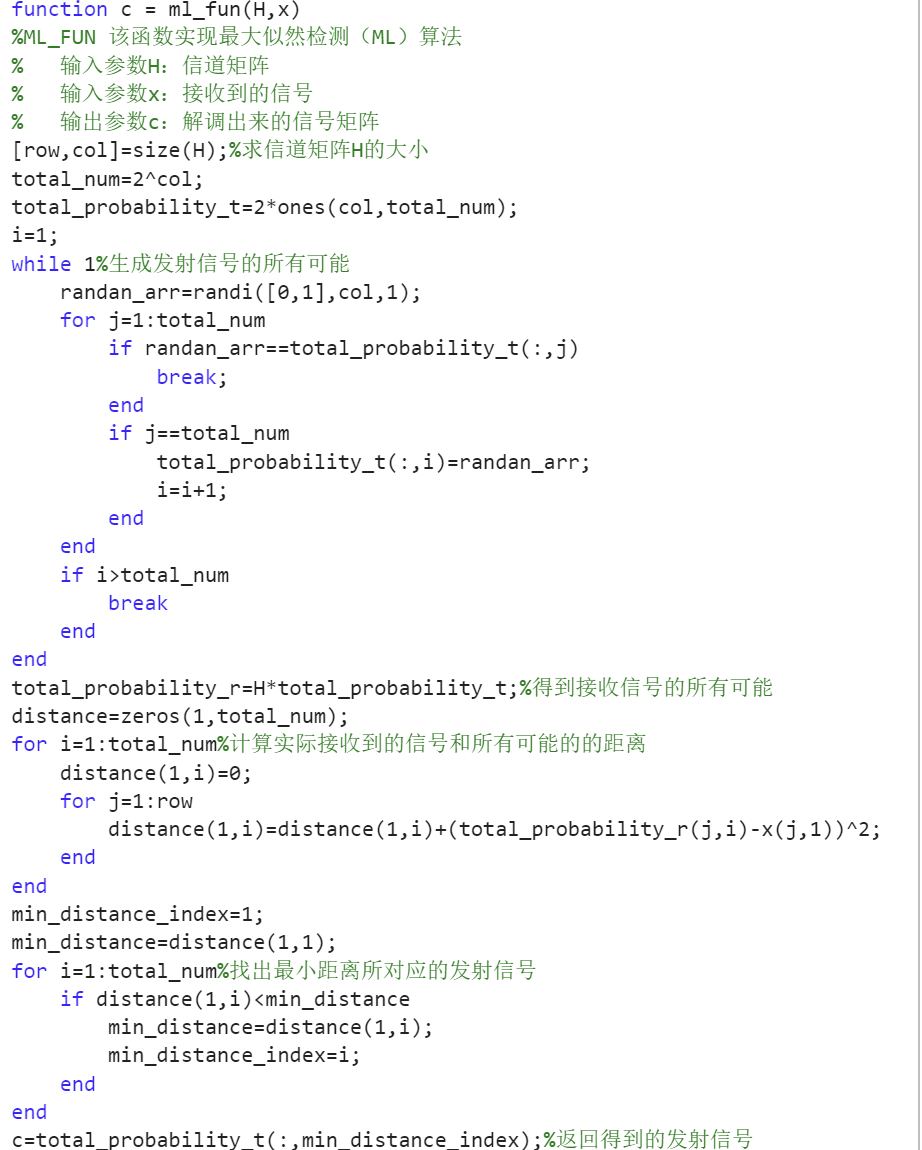
\includegraphics[width=0.8\textwidth]{25.png}
		\caption{ML matlab代码}
	\end{figure}
	\subsection{仿真测试}
	利用与上述相同的方法,对ML算法和ZF算法进行误码率和误帧率测试,然后将两者进行比较分析。由于ML算法的计算量随着天线数目的增加呈现指数级增长,所以本部分只对这两者算法进行$n_T=4,n_R=6$,信噪比为0-20dB的仿真测试。
	\subsubsection{误码率测试}
	 $n_T=4,n_R=6$,信噪比为0-20dB,测试帧数为1000000,结果如图25
		\begin{figure}[h]
			\centering
			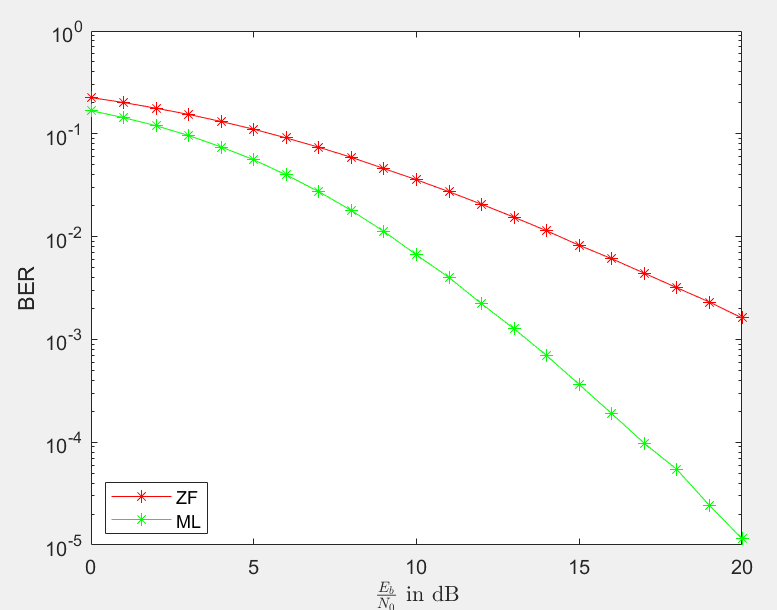
\includegraphics[width=0.5\textwidth]{26.png}
			\caption{$n_T=4,n_R=6$,信噪比为0-20dB,测试帧数为1000000的误码率测试结果图}
		\end{figure}
	\subsubsection{误帧率测试}
		$n_T=4,n_R=6$,信噪比为0-20dB,测试帧数为1000000,如图26
		\begin{figure}[h]			
			\centering
			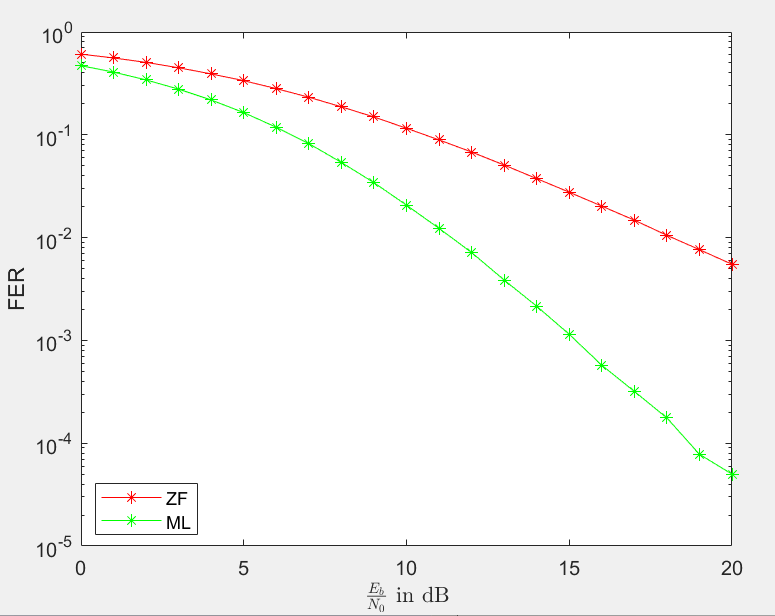
\includegraphics[width=0.5\textwidth]{27.png}
			\caption{$n_T=4,n_R=6$,信噪比为0-20dB,测试帧数为1000000的误帧率测试结果图}
		\end{figure}
	\subsubsection{结果分析}
	从图中可以看出,在相同的信噪比下,ML的误码率和误帧率对于ZF算法来说显著降低,主要原因是ZF算法计算了发送信号所有可能的集合,在理论上可以以最高的准确度找到发送信号,但是随着通道数的增加,信号的可能性指数增长,运算量急剧增大,所有在实际应用中,ML算法的应用范围受到了很大的限制,实用性不强。
	\section{对算法实现过程一些内容的补充}
	\subsection{自编写QR算法}
	在文中提到的许多算法中,多处需要用到QR分解,在上面的仿真实现中,都是直接调用了系统中的函数,下面尝试自己编写QR分解算法进行补充。\par 
	实现代码如图27,测试结果如图28,Q,R是使用自编写QR分解得到的结果;q,r是使用系统QR分解得到的结果。
	\begin{figure}[h]
		\centering
		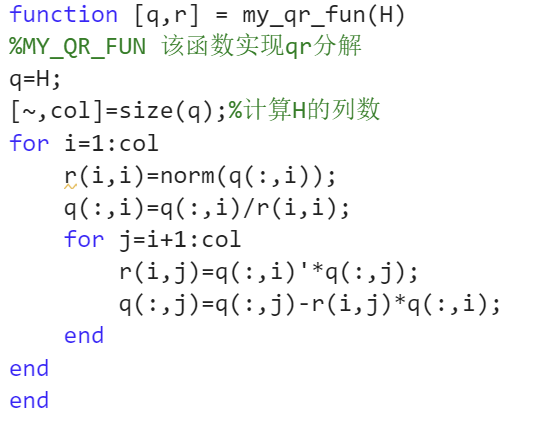
\includegraphics[width=0.5\textwidth]{28.png}
		\caption{自编写QR分解代码}
	\end{figure}
	\begin{figure}[h]
		\centering
		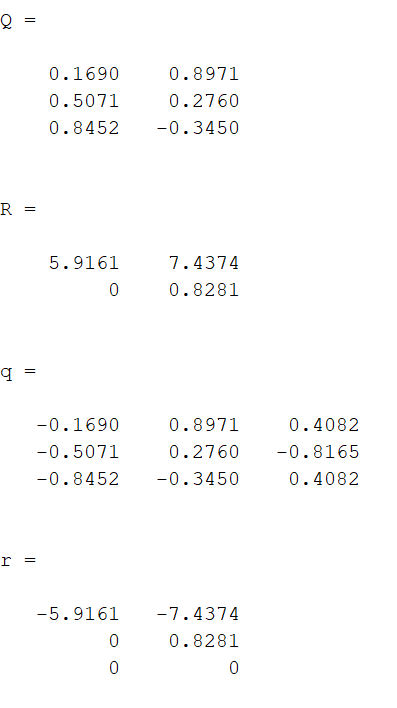
\includegraphics[width=0.3\textwidth]{29.png}
		\caption{自编写QR分解测试结果}
	\end{figure}
	\subsection{将实数信号拓展到复数信号}
	\subsubsection{原理}
	在上述的讨论中,我们假定一帧信号所携带的信息只有1比特,即信号的可能性只有0和1。这里考虑发射天线发射的信号为复数,即$c=ai+bj$,这样,一帧信号所携带的信息则变为2比特。信号在接收端经过信道矩阵H处理后,所得到的x仍为复数。所得到的信号经过解调后,对其进行复数平面的欧式最小距离判决,即可的到发射信号。\par 
	在matlab中,复数的运算已经有了定义,所以将实数信号拓展为复数信号十分方便,只需要更改判决方式即可。
	\subsubsection{实现}
	这里将ZF算法重写,使其能够对复数信号进行解调,其与解调实数信号主要的不同在于对信号的判决方式不同。重写的matlab代码如图29。\par
	\begin{figure}[h]
		\centering
		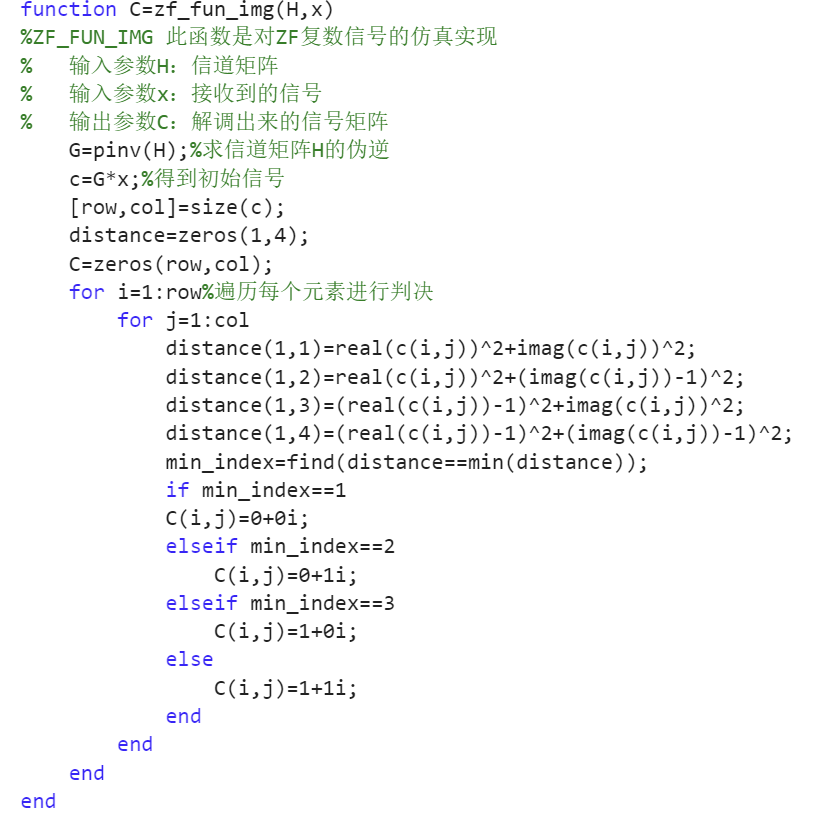
\includegraphics[width=0.6\textwidth]{30.png}
		\caption{适用于复数信号的ML matlab代码}
	\end{figure}
	因此我们可以看出,在matlab中,要实现从实数到复数的转变,只需要更改算法的判决方式即可。其他算法同理,因此不一一重写。
	\subsubsection{测试}
	我们采用与前文相同的测试方法,测试适用于实数的ZF算法和适用于复数的ZF算法的误码率,比较分析得到复数信号的优点。测试代码如图30。\par 
	\begin{figure}[h]
		\centering
		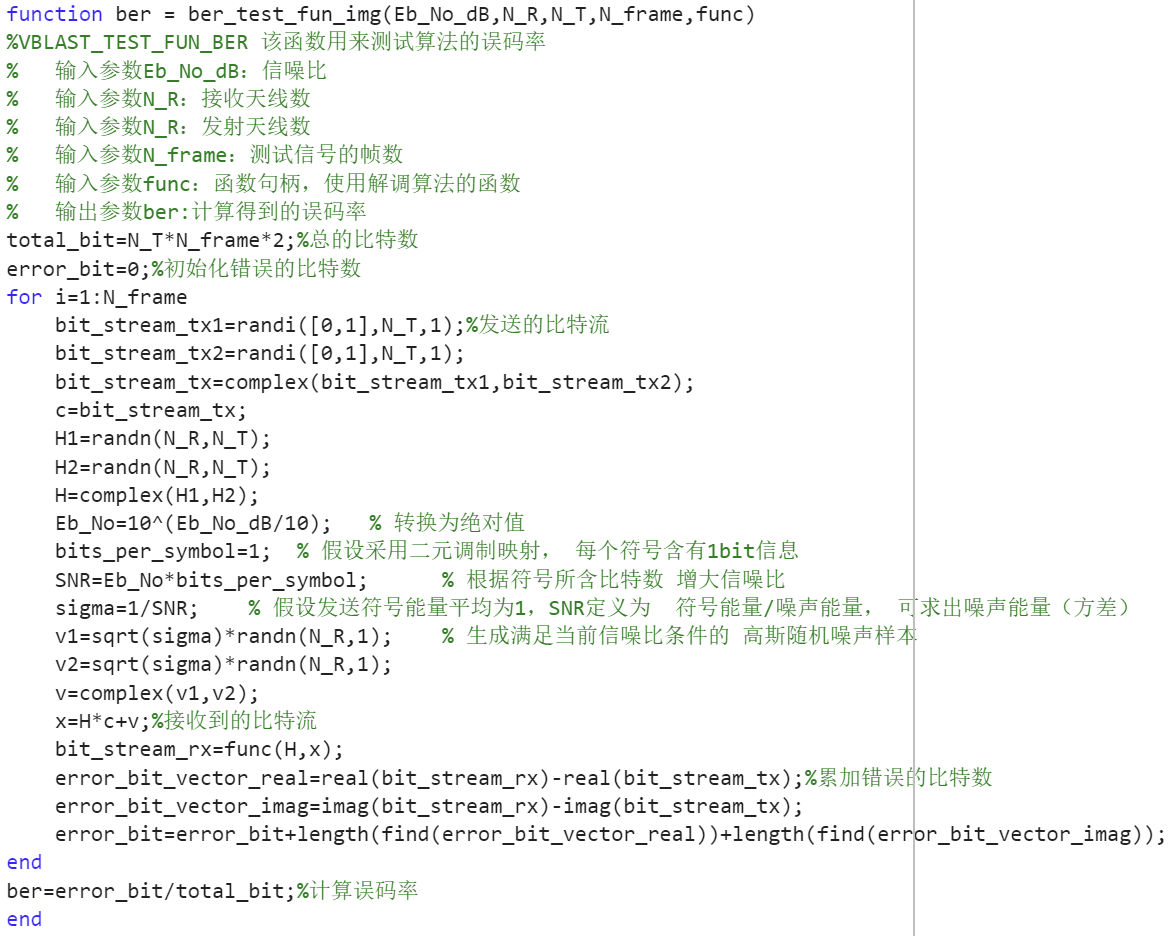
\includegraphics[width=0.7\textwidth]{31.png}
		\caption{测试复数信号代码}
	\end{figure}
	通过测试适用于实数的ZF算法和适用于复数的ZF算法在1000000帧时,信噪比在0-20dB之间的误码率,得到如图31和图32所示结果。
	\begin{figure}[h]
		\centering
		\begin{minipage}{0.4\textwidth}
			\centering
			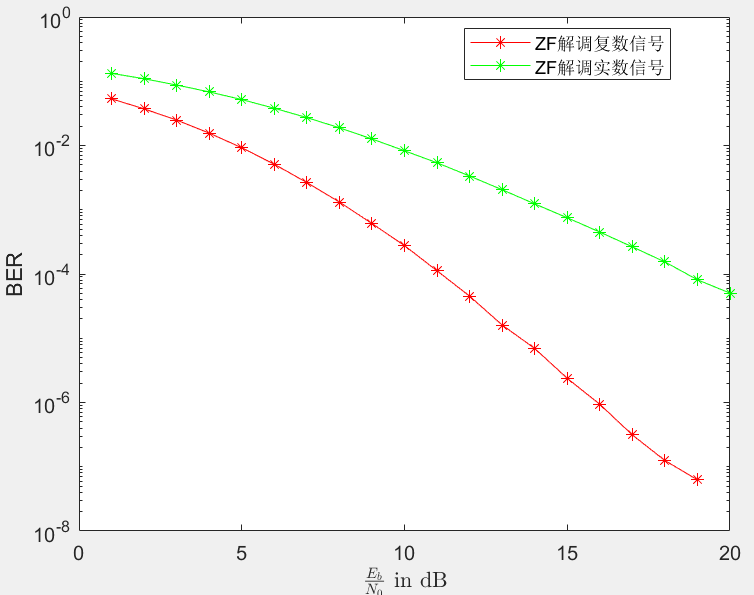
\includegraphics[width=\textwidth]{33.png}
			\caption{$n_T=8,n_R=12$,信噪比为0-20dB,测试帧数为1000000的误帧率测试结果图}
		\end{minipage}
		\qquad
		\begin{minipage}{0.4\textwidth}
			\centering
			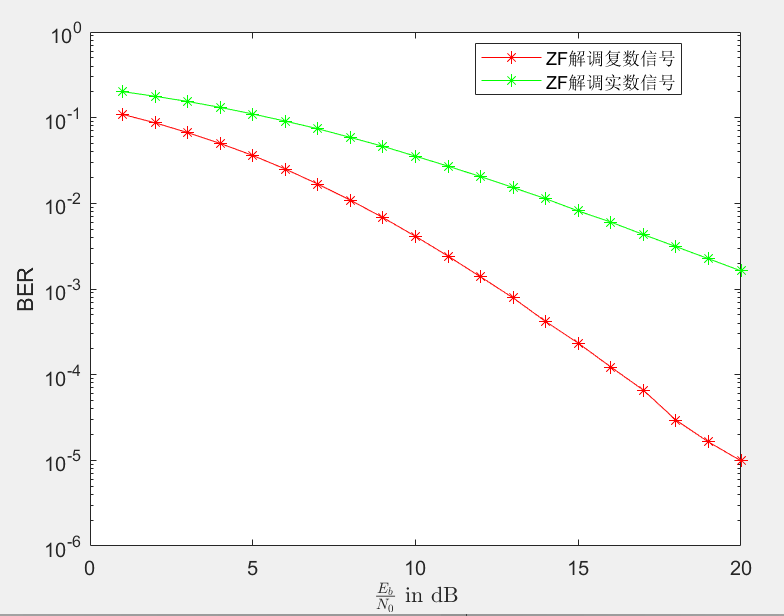
\includegraphics[width=\textwidth]{32.png}
			\caption{$n_T=4,n_R=6$,信噪比为0-20dB,测试帧数为1000000的误帧率测试结果图}
		\end{minipage}
	\end{figure}
	通过观察实验结果,发现复数信号比实数信号的误码率更低,因为复数信号相比实数信号携带的信息更多,因此使用复数信号可以提供更大的灵活性和描述能力,但有时也会增加计算复杂度。
	\section{对算法复杂度的测试}
	\subsection{说明}
	在上面的算法实现过程中,着重考虑了各个算法的误码率,对各个算法的复杂度只是进行了理论的分析,并没有进行测试比较。
	这里对算法复杂度进行重新测试,作为补充。
	\subsection{对论文1中各个算法复杂度测试}
	假设发射天线数为8,接收天线数为12分别用V-BLAST、QRD、SQRD算法来处理10000帧信号,计算他们所用的时间,即可比较他们的计算复杂度,测试结果如图33
	\begin{figure}[h]
		\centering
		\begin{tabular}{|c|c|c|c|}
			\hline
			算法 & V-BLAST & QRD & SQRD \\
			\hline
			时间(秒) & 27.210518 & 2.409250 & 6.079538 \\
			\hline 
		\end{tabular}
		\caption{对论文1各个算法复杂度测试}
	\end{figure}
	\subsection{对论文2中各个算法复杂度测试}
	假设发射天线数为8,接收天线数为12分别用ZF、MMSE、MMSE-QRD、MMSE-SQRD算法来处理10000帧信号,计算他们所用的时间,即可比较他们的计算复杂度,测试结果如图34
	\begin{figure}[h]
		\centering
		\begin{tabular}{|c|c|c|c|c|}
			\hline
			算法 & ZF & MMSE & MMSE-QRD & MMSE-SQRD \\
			\hline
			时间(秒) & 6.789264 & 1.594085 & 4.168950 & 6.960158 \\
			\hline 
		\end{tabular}
		\caption{对论文2各个算法复杂度测试}
	\end{figure}
	\subsection{总结}
	在matlab中对这几个代码的测试,基本符合理论分析,但是在对MMSE算法的测试中,发现MMSE算法所用的时间较短,不符合理论分析,可能的原因是matlab对矩阵求逆运算的优化。另一方面,在模拟的过程中,很难准确计算出算法运算的时间,因为包含了一些其他的函数处理,导致了结果不太精准。
	\section{总结与思考}
	在这次大作业中,最大的收获是如何进行通信仿真。从一开始的对论文无处下手,再到慢慢看懂里面的算法,最后用matlab代码将其实现出来。一步步地掌握了仿真的要领。\par 
	以本次作业的MIMO系统为例,要将这样的一个系统,用matlab表征出来。首先是对系统的理解,即对四个系统量$c,x,v,H$的理解,如何用0和1代表信号,用矩阵的线性运算模拟解调过程,最后用不同的算法由接收信号得到发射信号。在算法实现过程中,最难的是看懂论文中对算法的描述,以及给出的伪代码图。不同的论文。可能对同一变量的描述不一样,因此要学会用统一的符号进行转述。\par 
	本文对论文中所有提到的算法都进行了复现并都在不同的$n_R,n_T$下测试了误码率和误帧率,并且还实现了最大似然检测算法。在算法的实现过程中,遇到了许多困难,例如流程图中的许多符号看不懂,以及进行排序时如何记录排列顺序等等。但最后都在同学的帮助下解决了。虽然都对算法进行了复现,但是在进行编程的过程中,有些地方处理地比较笨拙,导致代码繁琐,因此还需改进。\par 
	本文用matlab进行仿真,实现起来可能比较简单,因为matlab丰富的函数库、矩阵运算以及能够实时可见的工作区变量,为算法的复现带来了很大便利。通过使用matlab中的串行计算工具包,极大地减少了仿真测试的时间,使得能够在短时间内获得大量的数据。\par 
	通过本次对MIMO系统中许多算法的仿真测试,我对MIMO通信系统有了较深的理解,同时也深刻感受到了在计算机科学计算中,数值计算方法是一门很大的学问。课堂上学习到的知识,在这里有了更深的体会。
\end{document}